% Template of basic phisics experiment 基于 article template，在此基础上做修改
% 设定文章编码类型，正文字号为五号则 zihao=5，正文字号为小四则 zihao=-4
\documentclass[zihao=5, UTF8]{article}		


% 自定义宏定义
\def\N{\mathbb{N}}
\def\F{\mathbb{F}}
\def\Z{\mathbb{Z}}
\def\Q{\mathbb{Q}}
\def\R{\mathbb{R}}
\def\C{\mathbb{C}}
\def\T{\mathbb{T}}
\def\S{\mathbb{S}}
\def\A{\mathbb{A}}
\def\I{\mathscr{I}}
\def\d{\mathrm{d}}
\def\p{\partial}


% 物理实验报告所需的其它宏包
\usepackage{ulem}   % \uline 下划线支持

% 导入基本宏包
\usepackage[UTF8]{ctex}     % 设置文档为中文语言
\usepackage[colorlinks, linkcolor=blue, anchorcolor=blue, citecolor=blue, urlcolor=blue]{hyperref}  % 宏包：自动生成超链接 (此宏包与标题中的数学环境冲突)
% \usepackage{docmute}    % 宏包：子文件导入时自动去除导言区，用于主/子文件的写作方式，\include{./51单片机笔记}即可。注：启用此宏包会导致.tex文件capacity受限。
\usepackage{amsmath}    % 宏包：数学公式
\usepackage{mathrsfs}   % 宏包：提供更多数学符号
\usepackage{amssymb}    % 宏包：提供更多数学符号
\usepackage{pifont}     % 宏包：提供了特殊符号和字体
\usepackage{extarrows}  % 宏包：更多箭头符号

% 列表环境设置
\usepackage{enumitem}   % 宏包：列表环境设置
    \setlist[enumerate]{itemsep=0pt, parsep=0pt, topsep=0pt, partopsep=0pt, leftmargin=3.5em} 
    \setlist[itemize]{itemsep=0pt, parsep=0pt, topsep=0pt, partopsep=0pt, leftmargin=3.5em}
    \newlist{circledenum}{enumerate}{1} % 创建一个新的枚举环境  
    \setlist[circledenum,1]{  
        label=\protect\circled{\arabic*}, % 使用 \arabic* 来获取当前枚举计数器的值，并用 \circled 包装它  
        ref=\arabic*, % 如果需要引用列表项，这将决定引用格式（这里仍然使用数字）
        itemsep=0pt, parsep=0pt, topsep=0pt, partopsep=0pt, leftmargin=3.5em
    }  
% 文章页面 margin 设置
\usepackage[a4paper]{geometry}  % 宏包：文章页面 margin 设置
    \geometry{top=0.75in}
    \geometry{bottom=0.75in}
    \geometry{left=0.75in}
    \geometry{right=0.75in}   % 设置上下左右页边距
    \geometry{marginparwidth=1.75cm}    % 设置边注距离（注释、标记等）

% 自定义数学环境
\usepackage{amsthm} % 宏包：数学环境配置
% theorem-line 环境自定义
    \newtheoremstyle{MyLineTheoremStyle}% <name>
        {11pt}% <space above>
        {11pt}% <space below>
        {}% <body font> 使用默认正文字体
        {}% <indent amount>
        {\bfseries}% <theorem head font> 设置标题项为加粗
        {：}% <punctuation after theorem head>
        {.5em}% <space after theorem head>
        {\textbf{#1}\thmnumber{#2}\ \ (\,\textbf{#3}\,)}% 设置标题内容顺序
    \theoremstyle{MyLineTheoremStyle} % 应用自定义的定理样式
    \newtheorem{LineTheorem}{Theorem.\,}
% theorem-block 环境自定义
    \newtheoremstyle{MyBlockTheoremStyle}% <name>
        {11pt}% <space above>
        {11pt}% <space below>
        {}% <body font> 使用默认正文字体
        {}% <indent amount>
        {\bfseries}% <theorem head font> 设置标题项为加粗
        {：\\ \indent}% <punctuation after theorem head>
        {.5em}% <space after theorem head>
        {\textbf{#1}\thmnumber{#2}\ \ (\,\textbf{#3}\,)}% 设置标题内容顺序
    \theoremstyle{MyBlockTheoremStyle} % 应用自定义的定理样式
    \newtheorem{BlockTheorem}[LineTheorem]{Theorem.\,} % 使用 LineTheorem 的计数器
% definition 环境自定义
    \newtheoremstyle{MySubsubsectionStyle}% <name>
        {11pt}% <space above>
        {11pt}% <space below>
        {}% <body font> 使用默认正文字体
        {}% <indent amount>
        {\bfseries}% <theorem head font> 设置标题项为加粗
        {：\\ \indent}% <punctuation after theorem head>
        {0pt}% <space after theorem head>
        {\textbf{#3}}% 设置标题内容顺序
    \theoremstyle{MySubsubsectionStyle} % 应用自定义的定理样式
    \newtheorem{definition}{}


% 有色文本框及其设置
\usepackage[dvipsnames,svgnames]{xcolor}    %设置插入的文本框颜色
\usepackage[strict]{changepage}     % 提供一个 adjustwidth 环境
\usepackage{framed}     % 实现方框效果
    \definecolor{graybox_color}{rgb}{0.95,0.95,0.96} % 文本框颜色。修改此行中的 rgb 数值即可改变方框纹颜色，具体颜色的rgb数值可以在网站https://colordrop.io/ 中获得。（截止目前的尝试还没有成功过，感觉单位不一样）（找到喜欢的颜色，点击下方的小眼睛，找到rgb值，复制修改即可）
    \newenvironment{graybox}{%
    \def\FrameCommand{%
    \hspace{1pt}%
    {\color{gray}\small \vrule width 2pt}%
    {\color{graybox_color}\vrule width 4pt}%
    \colorbox{graybox_color}%
    }%
    \MakeFramed{\advance\hsize-\width\FrameRestore}%
    \noindent\hspace{-4.55pt}% disable indenting first paragraph
    \begin{adjustwidth}{}{7pt}%
    \vspace{2pt}\vspace{2pt}%
    }
    {%
    \vspace{2pt}\end{adjustwidth}\endMakeFramed%
    }

% 各级标题自定义设置
\usepackage{titlesec}   
    % section标题自定义设置 
    \titleformat{\section}[hang]{\normalfont\huge\bfseries\centering}{第\,\thesection\,部分}{20pt}{}
    % subsection标题自定义设置 
    \titleformat{\subsection}[hang]{\normalfont\Large\bfseries}{\,\thesubsection\,}{8pt}{}
    % subsubsection标题自定义设置
    \titleformat{\subsubsection}[hang]{\normalfont\large\bfseries}{\,\thesubsubsection\,}{6pt}{}

% 外源代码插入设置
\usepackage{matlab-prettifier}
    \lstset{
        style=Matlab-editor,  % 继承matlab代码颜色等
    }
\usepackage[most]{tcolorbox} % 引入tcolorbox包 
\usepackage{listings} % 引入listings包
    \tcbuselibrary{listings, skins, breakable}
    \lstdefinestyle{matlabstyle}{
        language=Matlab,
        basicstyle=\small,
        breakatwhitespace=false,
        breaklines=true,
        captionpos=b,
        keepspaces=true,
        numbers=left,
        numbersep=15pt,
        showspaces=false,
        showstringspaces=false,
        showtabs=false,
        tabsize=2
    }
    \newtcblisting{matlablisting}{
        arc=0pt,
        top=0pt,
        bottom=0pt,
        left=1mm,
        listing only,
        listing style=matlabstyle,
        breakable,
        colback=white   % 选一个合适的颜色
    }

% table 支持
\usepackage{booktabs}   % 宏包：三线表
\usepackage{tabularray} % 宏包：表格排版
\usepackage{longtable}  % 宏包：长表格
\usepackage{tabularx}  % 宏包：宽表格
\usepackage{multirow}  % 宏包：表格中一格显示多个项目

% figure 设置
\usepackage{graphicx}  % 支持 jpg, png, eps, pdf 图片 
\usepackage{svg}       % 支持 svg 图片
    \svgsetup{
        % 指向 inkscape.exe 的路径
        inkscapeexe = C:/aa_MySame/inkscape/bin/inkscape.exe, 
        % 一定程度上修复导入后图片文字溢出几何图形的问题
        inkscapelatex = false                 
    }


% 图表进阶设置
\usepackage{float}     % 图表位置浮动设置 
\usepackage{caption}    % 图注、表注
    \captionsetup[figure]{name=图}  
    \captionsetup[table]{name=表}
    \captionsetup{labelfont=bf, font=small}

% 文章默认字体设置
    \usepackage{fontspec}   % 宏包：字体设置
       \setmainfont{SimSun}    % 设置中文字体为宋体字体
      \setCJKmainfont[AutoFakeBold=3]{SimSun} % 设置加粗字体为 SimSun 族，AutoFakeBold 可以调整字体粗细^     \setmainfont{Times New Roman} % 设置英文字体为Times New Roman


% 其它设置
    % equation 公式编号设置
        \makeatletter  
        \renewcommand{\theequation}{\thesection.\arabic{equation}}  
        \makeatother
    % 脚注设置
        \renewcommand\thefootnote{\ding{\numexpr171+\value{footnote}}}
    % 参考文献引用设置
        \bibliographystyle{unsrt}   % 设置参考文献引用格式为unsrt
        \newcommand{\upcite}[1]{\textsuperscript{\cite{#1}}}     % 自定义上角标式引用
    % 文章序言设置
        \newcommand{\cnabstractname}{序言}
        \newenvironment{cnabstract}{%
            \par\Large
            \noindent\mbox{}\hfill{\bfseries \cnabstractname}\hfill\mbox{}\par
            \vskip 2.5ex
            }{\par\vskip 2.5ex}


% 页眉页脚设置
\usepackage{fancyhdr}   %宏包：页眉页脚设置
    \pagestyle{fancy}
    \fancyhf{}
    \cfoot{\thepage}
    \renewcommand\headrulewidth{1pt}
    \renewcommand\footrulewidth{0pt}
    \rhead{\bfseries 分组序号: YK04-2}    
    \chead{《基础物理实验》实验报告,\ 韩初晓,\ 2023K8009908002}
    \lhead{2024.12.19}

% 文档信息设置
%\title{这里是标题\\The Title of the Report}
%\author{丁毅\\ \footnotesize 中国科学院大学，北京 100049\\ Yi Ding \\ %\footnotesize University of Chinese Academy of Sciences, Beijing %100049, China}
%\date{\footnotesize 2024.8 -- 2025.1}

% 开始编辑文章

\begin{document}
\noindent\begin{flushright}
    \zihao{2}{分组序号: YK04-2}
\end{flushright}

\setCJKfamilyfont{boldsong}[AutoFakeBold = {2.17}]{SimSun}
\newcommand*{\boldsong}{\CJKfamily{boldsong}}


\begin{center}\large
    \noindent{\Huge\bfseries\boldsong《基础物理实验》实验报告 }
    \\\vspace{0.4cm}
    \noindent\textit{
        \textbf{\boldsong 实验名称：}\uline{\hspace{1.7cm} 虚拟仪器\hspace{1.7cm}}\hspace{0.4cm} 
        指导教师：\uline{\hspace{1.0cm}石澔玙\hspace{1.0cm}}}
    \\\vspace{0.1cm}
    \noindent\textit{
        姓名：\uline{\,\,\,韩初晓\,\,\,}\hspace{0.2cm}
        学号：\uline{\,\,\,{\upshape 2023K8009908002}\,\,\,}\hspace{0.2cm}
        专业：\uline{\,\,\,计算机科学与技术\,\,\,}\hspace{0.2cm}
        班级：\uline{\,\,\,\upshape{2306}\,\,\,}}
    \\\vspace{0.1cm}
    \noindent\textit{
        实验日期：\uline{\,\,{\upshape 2024.12.19}\,\,}\hspace{0.2cm}
        实验地点：\uline{\,\,\,教学楼{\upshape702}\,\,\,}\hspace{0.2cm}
        是否调课/补课：\uline{\hspace{0.5cm}否\hspace{0.5cm}}\hspace{0.2cm}
        成绩：\uline{\hspace{2cm}}}
\end{center}
% \vspace{-0.2cm}
\noindent\rule{\textwidth}{0.1em}   % 分割线

% 控制目录不换页
\vspace{1cm}
\setcounter{tocdepth}{2}  % 目录深度为 2（不显示 subsubsection）
\noindent\begin{minipage}{\textwidth}\centering
\tableofcontents\thispagestyle{fancy}   % 显示页码、页眉等   
\end{minipage}  
\newpage

\section{实验目的}\thispagestyle{fancy} 

\begin{enumerate}
    \item 了解虚拟仪器的概念；
    \item 了解图形化编程语言 LabVIEW，学习简单的 LabVIEW 编程；
    \item 完成伏安法测电阻的虚拟仪器设计。
\end{enumerate}

\section{实验仪器}

\begin{itemize}
    \item 计算机（含操作系统）；
    \item LabVIEW 2014；
    \item NI ELVIS II+；
    \item 导线若干；
    \item 元件盒一个（包括：
    \begin{itemize}
        \item 100\(\, \Omega\) 标准电阻一个；
        \item 待测电阻 1 k\(\, \Omega\) 和 51\(\, \Omega\) 各一个；
        \item 稳压二极管一个；
    \end{itemize}
    ）；
    \item 热电偶等元件。
\end{itemize}


\section{实验原理}

\subsection{虚拟仪器的硬件}

本实验使用的硬件平台包括计算机和美国国家仪器公司（NI）的教学实验室虚拟仪器套件 NI ELVIS II+，它集成了多个功能模块，如示波器、数字万用表、函数发生器等，支持通过 USB 与计算机连接。平台包括 8 通道差分模拟输入、24 路数字 I/O、2 通道示波器、函数发生器等多项功能，且通过 LabVIEW 软件进行编程和控制。

\subsection{虚拟仪器的软件}

虚拟仪器系统使用 LabVIEW 平台进行开发，它是基于图形化编程语言的工具，使得用户通过设计流程图进行编程，简化了传统编程的复杂性。LabVIEW 中的虚拟仪器（VI）包括前面板、程序框图和图标/连线板。前面板用于设置输入和显示输出，程序框图则实现仪器的功能和控制。

\subsection{利用虚拟仪器测量伏安特性}

本实验使用虚拟仪器测量伏安特性，利用模拟输出通道供电，并通过模拟输入通道测量电压和电流。实验中，电压从 0V 逐渐增加，每次电压变化后记录电流与电压的值，最终通过线性拟合计算待测电阻。测量可通过单端或差分输入方式进行。
利用虚拟仪器测量伏安特性的电路图如图 \ref{fig:va_measurement_principle} 所示：

\begin{figure}[H]
    \centering
    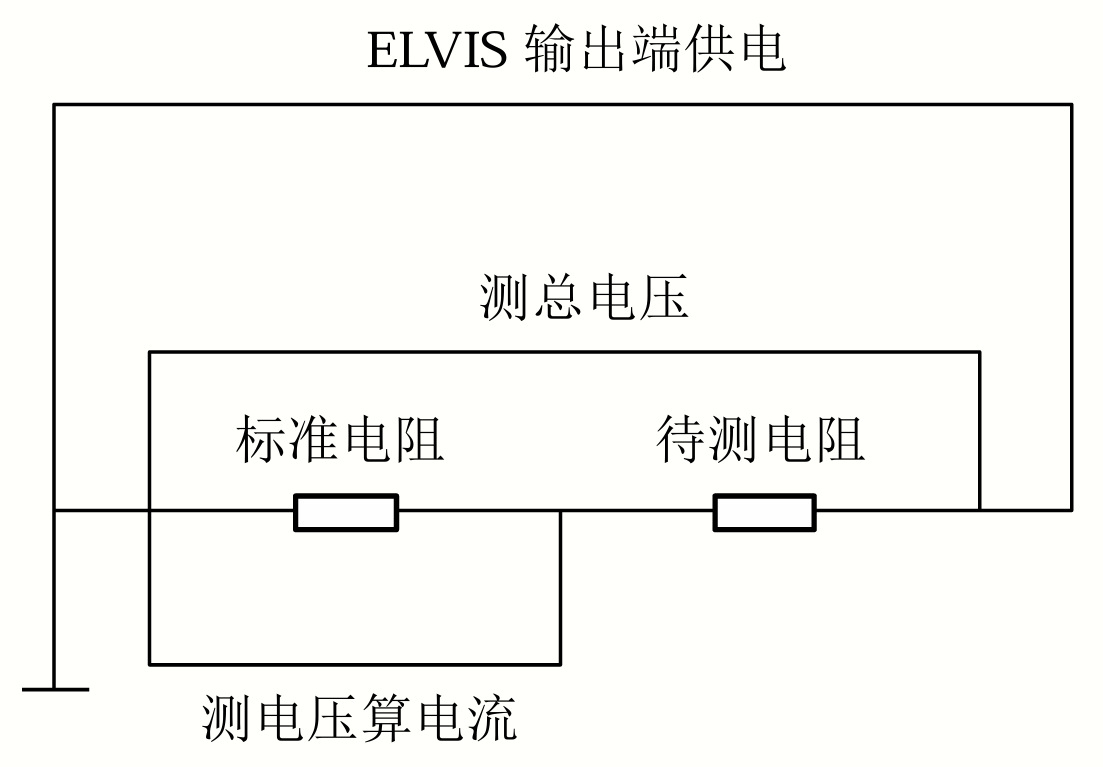
\includegraphics[width=0.6\textwidth]{./v_a_measurement_principle.png}
    \caption{虚拟仪器测量伏安特性的电路图}
    \label{fig:va_measurement_principle}
\end{figure}

\section{实验内容}

\subsection{编写一个温度测量程序}

我们假设传感器的输出电压与温度成正比，可以编写一个程序来根据输入电压计算温度值。程序允许切换摄氏温度与华氏温度的显示，并通过输入控件模拟采集的电压值。前面板包括温度计、滑动杆开关、数值显示和输入控件，程序框图中使用函数计算温度并选择显示单位。最后，通过运行程序并调整电压值来观察温度变化，验证程序功能。最终设计出的虚拟仪器前面板和程序框图如下图所示：

\begin{figure}[H]
    \centering
    \includegraphics[width=\textwidth]{./exp_2.JPG}
    \caption{温度测量程序的虚拟仪器设计}
    \label{fig:temperature_measurement}
\end{figure}

\subsection{创建一个电压输出和采集的程序}

首先，新建一个空白的 VI 并编写输出电压程序，通过 DAQmx 虚拟通道和“模拟输出”功能设置电压输出。然后，在程序框图中加入“DAQmx开始任务”、“DAQmx写入”和“DAQmx清除任务”节点，并创建一个 While 循环控制程序运行。接着，使用类似的方法编写电压采集程序，设置合适的输入控件，并将各个控件和函数连线。运行程序时，设置输出和输入通道，连接原型板，观察输出电压与测量电压的变化。最后，程序运行完毕后，点击停止按钮，保存文件并关闭程序。最终设计出的虚拟仪器前面板和程序框图如下图所示：

\begin{figure}[H]
    \centering
    \includegraphics[width=\textwidth]{./exp_3.JPG}
    \caption{电压输出和采集程序的虚拟仪器设计}
    \label{fig:voltage_output_measurement}
\end{figure}

\subsection{使用虚拟仪器测测量电阻的伏安特性}


首先，编写程序并创建前面板，添加一个 Express XY 图来显示电压-电流图，修改坐标轴标签为电流（A）和电压（V），并设置曲线模式为“点+线”。在前面板上添加多个数值型输入控件，如“输出电压步长”、“测量数据点数”、“标准电阻”和“时间间隔”，并为“时间间隔”控件设置单位标签为秒。接着，创建程序框图，使用顺序结构来控制程序的执行流程，包括电压输出、等待、测量电压和计算电流。为了逐渐改变电压并测量电阻，通过 While 循环控制电压变化，并使用移位寄存器和创建数组功能实时显示电压和电流数据。最后，使用线性拟合来计算电阻值，并整理前面板和程序框图中的各个控件和连线，保存程序。之后，正确连接外部电路并运行程序，测量并绘制两种不同大小阻值的电阻和稳压二极管的伏安特性曲线。

最终设计出的虚拟仪器前面板和程序框图如下图所示：

\begin{figure}[H]
    \centering
    \includegraphics[width=\textwidth]{./exp_4_interface.JPG}
    \caption{测量电阻的伏安特性的虚拟仪器前面板}
    \label{fig:resistance_measurement}
\end{figure}

\begin{figure}[H]
    \centering
    \includegraphics[width=\textwidth]{./exp_4_program.JPG}
    \caption{测量电阻的伏安特性的虚拟仪器程序框图}
    \label{fig:resistance_measurement_program}
\end{figure}

面包板上的电路示意图如图 \ref{fig:breadboard_circuit} 所示：

\begin{figure}[H]
    \centering
    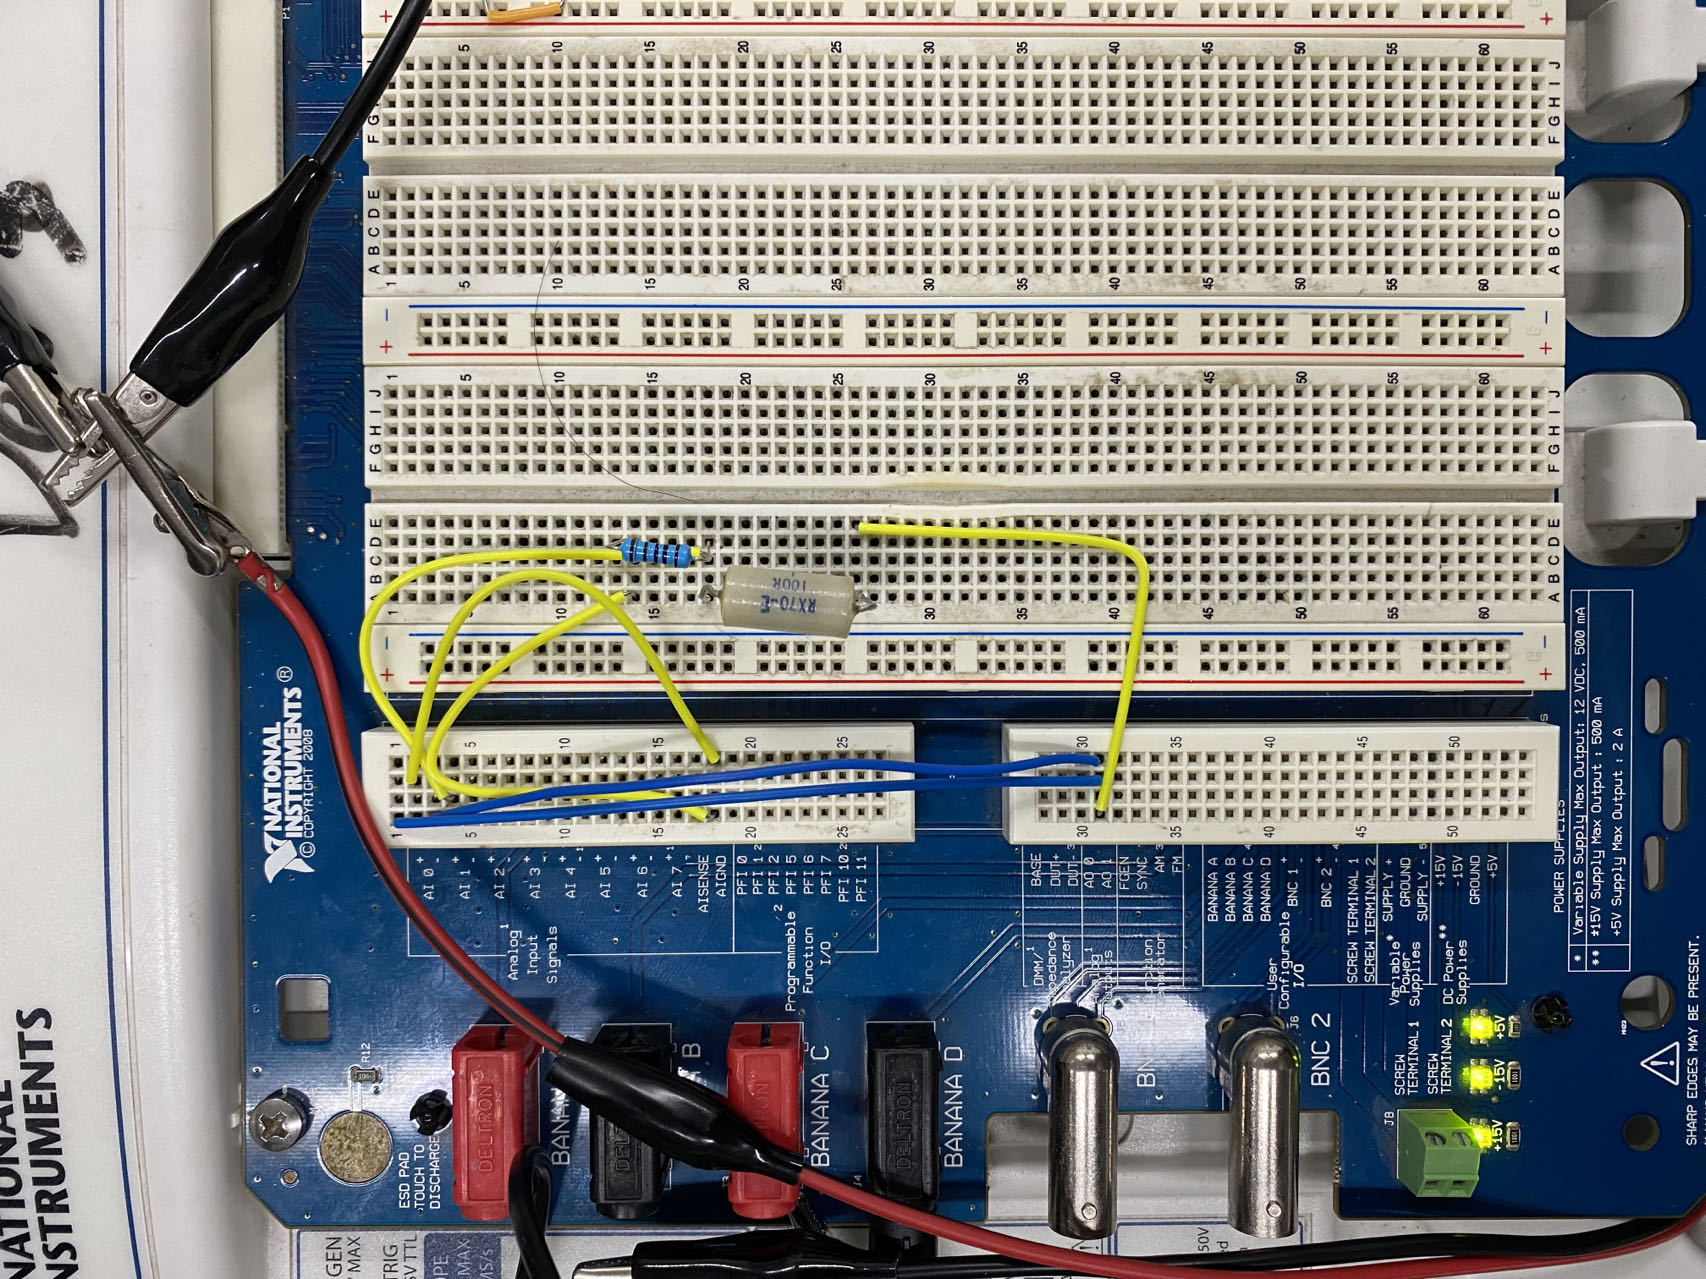
\includegraphics[width=0.6\textwidth]{./breadboard_circuit.JPG}
    \caption{测量电阻的伏安特性的电路示意图}
    \label{fig:breadboard_circuit}
\end{figure}

测量 51 \(\, \Omega\) 电阻的伏安特性曲线如图 \ref{fig:51ohm_va_curve} 所示：

\begin{figure}[H]
    \centering
    \includegraphics[width=\textwidth]{./exp_4_51.JPG}
    \caption{测量 51 \(\, \Omega\) 电阻的伏安特性曲线}
    \label{fig:51ohm_va_curve}
\end{figure}

伏安特性表如下：

\begin{longtable}{|c|c|c|c|c|c|c|}
\hline
\textbf{序号} & 1 & 2 & 3 & 4 & 5 & 6 \\
\hline
\textbf{电压 (V)} & -0.000322004 & 0.0164222 & 0.0338104 & 0.0499106 & 0.0669768 & 0.083721 \\
\hline
\textbf{电流 (A)} & 3.27E-06 & 0.00032849 & 0.000650494 & 0.000988598 & 0.00131704 & 0.00163905 \\
\hline
\textbf{序号} & 7 & 8 & 9 & 10 & 11 & 12 \\
\hline
\textbf{电压 (V)} & 0.0998212 & 0.117209 & 0.134598 & 0.150698 & 0.168086 & 0.184508 \\
\hline
\textbf{电流 (A)} & 0.00198037 & 0.00229915 & 0.00263082 & 0.00295926 & 0.00328449 & 0.00362259 \\
\hline
\textbf{序号} & 13 & 14 & 15 & 16 & 17 & 18 \\
\hline
\textbf{电压 (V)} & 0.200931 & 0.217031 & 0.234419 & 0.251485 & 0.268873 & 0.284974 \\
\hline
\textbf{电流 (A)} & 0.00394781 & 0.00427948 & 0.00460792 & 0.00493315 & 0.00525837 & 0.00559003 \\
\hline
\textbf{序号} & 19 & 20 & 21 & & & \\
\hline
\textbf{电压 (V)} & 0.301074 & 0.31814 & 0.335528 & & & \\
\hline
\textbf{电流 (A)} & 0.00592492 & 0.00625658 & 0.00657859 & & & \\
\hline
\caption{测量 51 \(\, \Omega\) 电阻的伏安特性表}
\end{longtable}

使用 Python 处理数据并绘制伏安特性曲线如图 \ref{fig:51ohm_va_curve_python} 所示：

\begin{figure}[H]
    \centering
    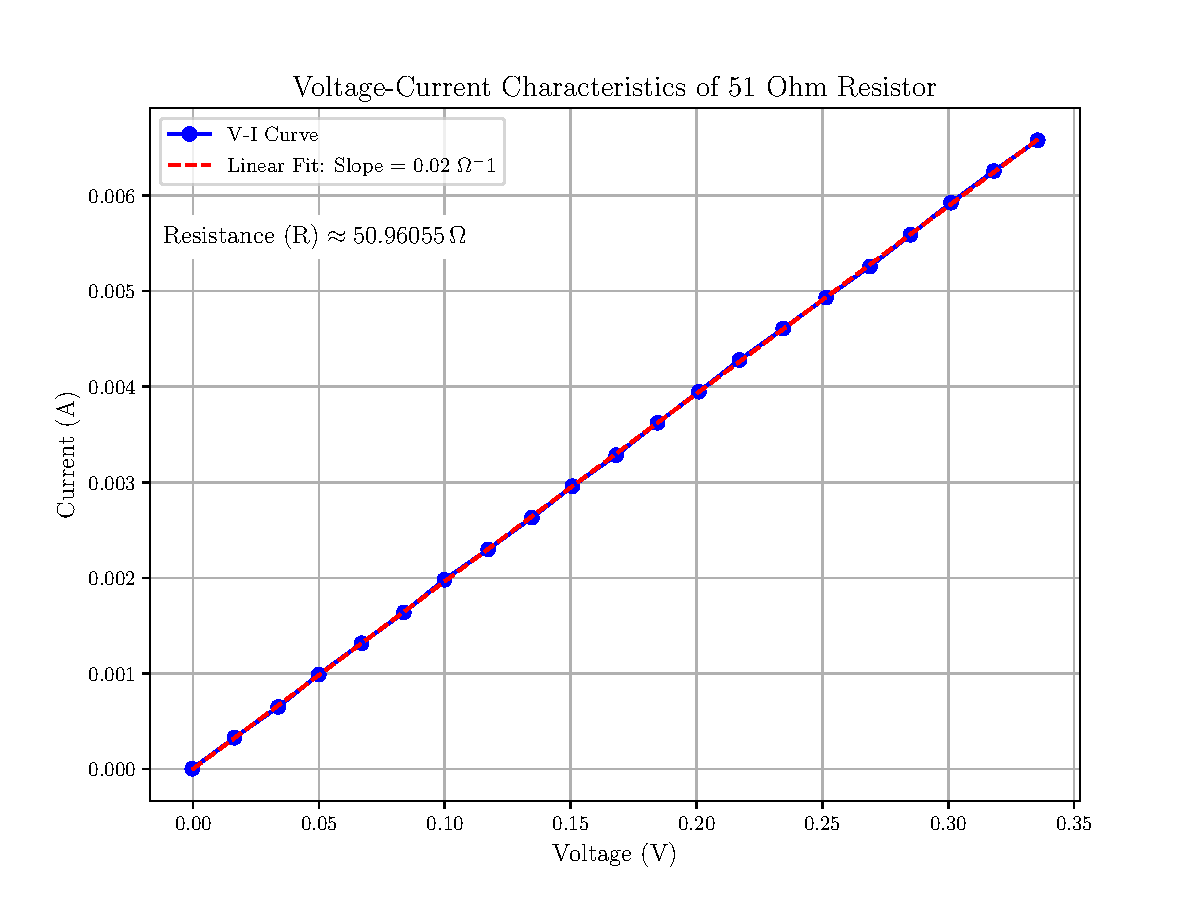
\includegraphics[width=0.6\textwidth]{./v_a_51.pdf}
    \caption{使用 Python 处理数据绘制 51 \(\, \Omega\) 电阻的伏安特性曲线}
    \label{fig:51ohm_va_curve_python}
\end{figure}

测量 1 k\(\, \Omega\) 电阻的伏安特性曲线如图 \ref{fig:1000ohm_va_curve} 所示：

\begin{figure}[H]
    \centering
    \includegraphics[width=\textwidth]{./exp_4_1000.JPG}
    \caption{测量 1 k\(\, \Omega\) 电阻的伏安特性曲线}
    \label{fig:1000ohm_va_curve}
\end{figure}

伏安特性表如下：

\begin{longtable}{|c|c|c|c|c|c|c|}
\hline
\textbf{序号} & 1 & 2 & 3 & 4 & 5 & 6 \\
\hline
\textbf{电压 (V)} & -0.00128802 & 0.452094 & 0.906763 & 1.36079 & 1.81482 & 2.26917 \\
\hline
\textbf{电流 (A)} & 1.29E-05 & 0.000466952 & 0.000914537 & 0.00137178 & 0.00182581 & 0.00227983 \\
\hline
\textbf{序号} & 7 & 8 & 9 & 10 & 11 & 12 \\
\hline
\textbf{电压 (V)} & 2.72287 & 3.17819 & 3.63125 & 4.08464 & 4.53867 & 4.99303 \\
\hline
\textbf{电流 (A)} & 0.0027403 & 0.0031911 & 0.00364835 & 0.0041056 & 0.00456284 & 0.00502009 \\
\hline
\textbf{序号} & 13 & 14 & 15 & 16 & 17 & 18 \\
\hline
\textbf{电压 (V)} & 5.44642 & 5.9011 & 6.35513 & 6.80885 & 7.26353 & 7.71693 \\
\hline
\textbf{电流 (A)} & 0.00547411 & 0.00592814 & 0.00638216 & 0.00683941 & 0.00729022 & 0.0077539 \\
\hline
\textbf{序号} & 19 & 20 & & & & \\
\hline
\textbf{电压 (V)} & 8.17098 & 8.62438 & 9.07875 & & & \\
\hline
\textbf{电流 (A)} & 0.00821115 & 0.00866517 & 0.00912242 & & & \\
\hline
\caption{测量 1 k\(\, \Omega\) 电阻的伏安特性表}
\end{longtable}

使用 Python 处理数据并绘制伏安特性曲线如图 \ref{fig:1000ohm_va_curve_python} 所示：

\begin{figure}[H]
    \centering
    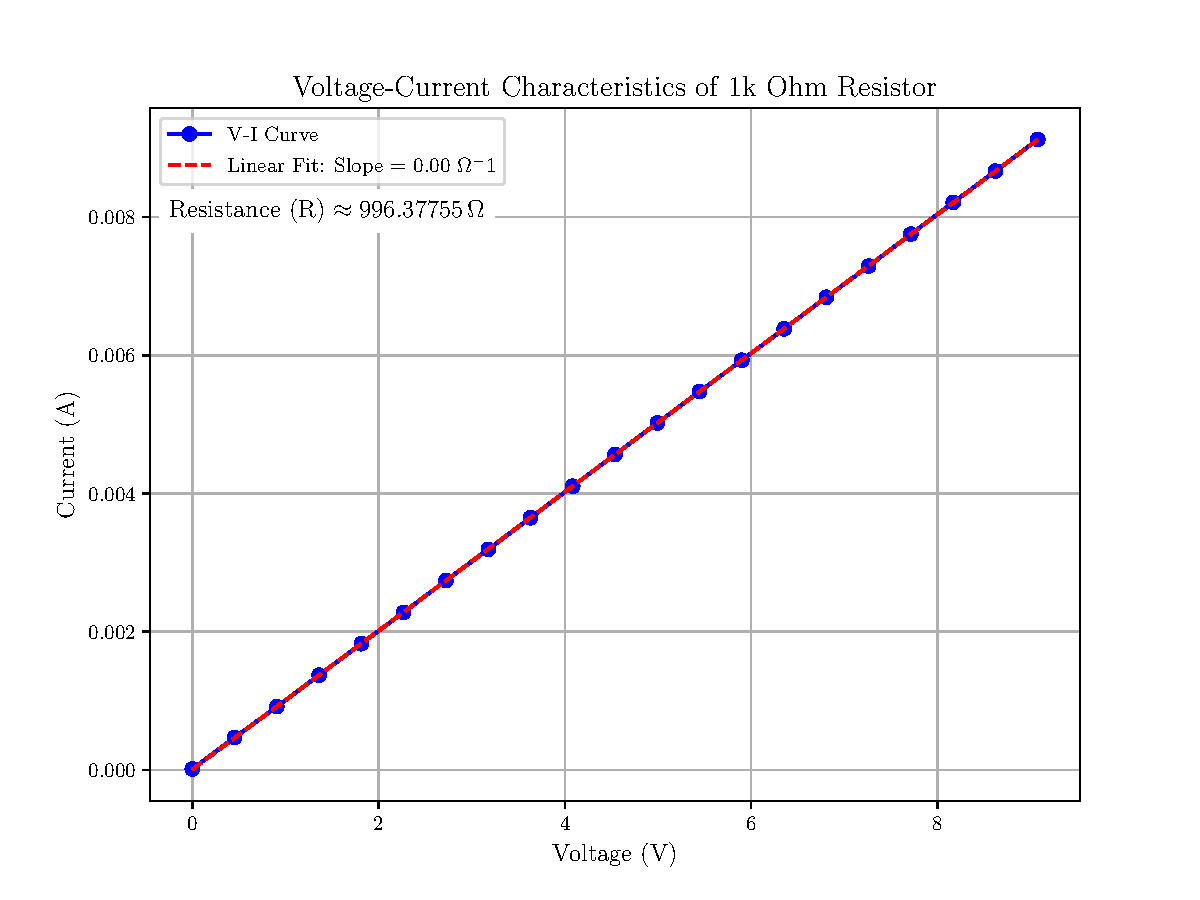
\includegraphics[width=0.6\textwidth]{./v_a_1000.pdf}
    \caption{使用 Python 处理数据绘制 1 k\(\, \Omega\) 电阻的伏安特性曲线}
    \label{fig:1000ohm_va_curve_python}
\end{figure}

测量稳压二极管的伏安特性曲线如图 \ref{fig:diode_va_curve} 所示：

\begin{figure}[H]
    \centering
    \includegraphics[width=\textwidth]{./exp_4_diode.JPG}
    \caption{测量稳压二极管的伏安特性曲线}
    \label{fig:diode_va_curve}
\end{figure}

稳压二极管的伏安特性表如下：

\begin{longtable}{|c|c|c|c|c|c|c|}
\hline
\textbf{序号} & 1 & 2 & 3 & 4 & 5 & 6 \\
\hline
\textbf{电压 (V)} & -0.00161002 & 0.0682648  & 0.13814    & 0.209303   & 0.278533   & 0.348086 \\
\hline
\textbf{电流 (A)} & 9.71E-06   & 1.29E-05   & 1.61E-05   & 3.27E-06   & 9.71E-06   & 1.29E-05 \\
\hline
\textbf{序号} & 7 & 8 & 9 & 10 & 11 & 12 \\
\hline
\textbf{电压 (V)} & 0.418605   & 0.487514   & 0.557711   & 0.624044   & 0.677818   & 0.709053 \\
\hline
\textbf{电流 (A)} & 1.61E-05   & 1.61E-05   & 2.26E-05   & 5.16E-05   & 0.000212569 & 0.000602194 \\
\hline
\textbf{序号} & 13 & 14 & 15 & 16 & 17 & 18 \\
\hline
\textbf{电压 (V)} & 0.726119   & 0.738999   & 0.747693   & 0.754778   & 0.762184   & 0.766048 \\
\hline
\textbf{电流 (A)} & 0.00112384 & 0.00169057 & 0.00229593 & 0.0029174  & 0.00354209 & 0.00419576 \\
\hline
\textbf{序号} & 19 & 20 & 21 & 22 & 23 & 24 \\
\hline
\textbf{电压 (V)} & 0.770556   & 0.773776   & 0.77764    & 0.780538   & 0.783759   & 0.786013 \\
\hline
\textbf{电流 (A)} & 0.00484621 & 0.00550309 & 0.00615354 & 0.00682009 & 0.00748342 & 0.00815641 \\
\hline
\textbf{序号} & 25 & 26 & 27 & 28 & 29 & 30 \\
\hline
\textbf{电压 (V)} & 0.788267   & 0.790843   & 0.794063   & 0.795995   & 0.797605   & 0.797927 \\
\hline
\textbf{电流 (A)} & 0.00882618 & 0.00949272 & 0.0101625  & 0.010829   & 0.0113829  & 0.0112637 \\
\hline
\textbf{序号} & 31 & 32 & & & & \\
\hline
\textbf{电压 (V)} & 0.796961   &            &            &            &            & \\
\hline
\textbf{电流 (A)} & 0.0111993  &            &            &            &            & \\
\hline
\caption{测量稳压二极管的伏安特性表}
\end{longtable}

使用 Python 处理数据并绘制伏安特性曲线如图 \ref{fig:diode_va_curve_python} 所示：

\begin{figure}[H]
    \centering
    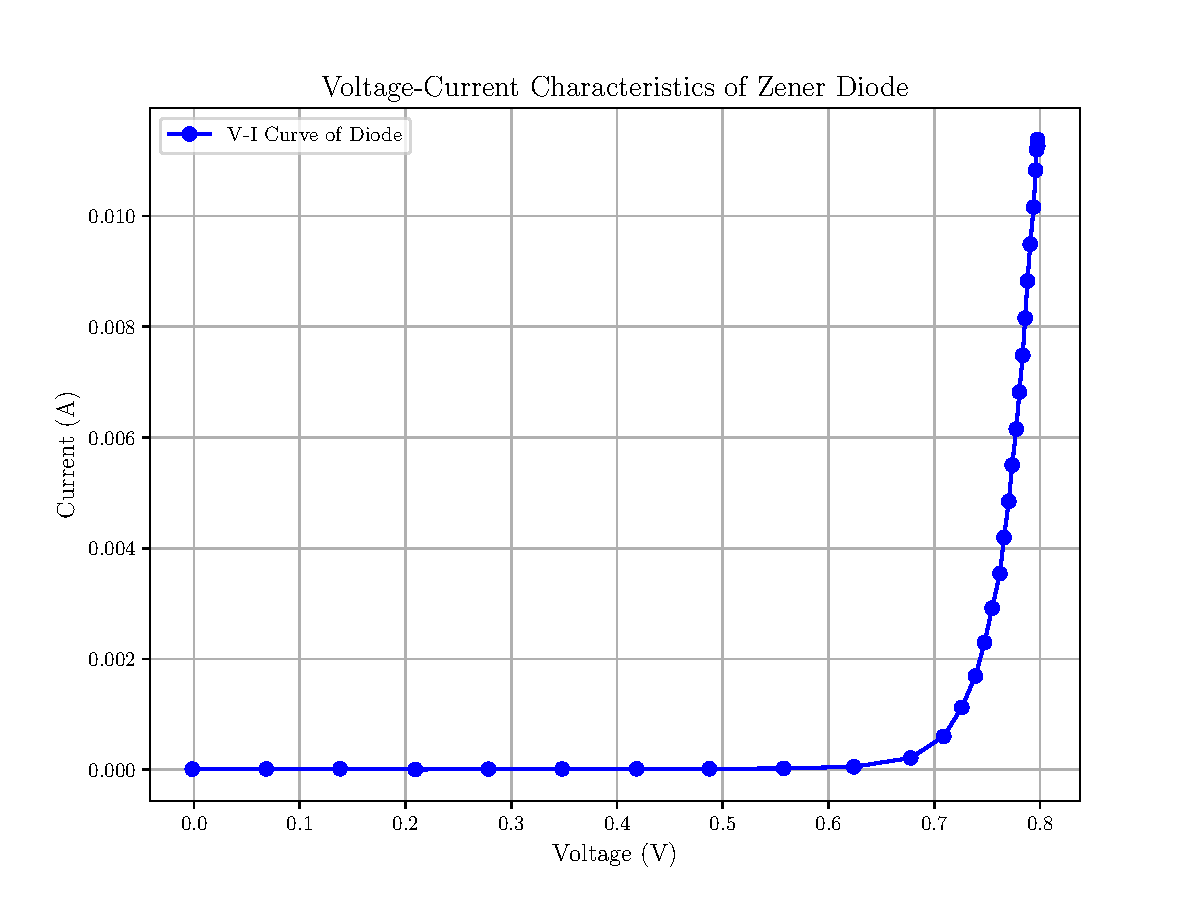
\includegraphics[width=0.6\textwidth]{./v_a_diode.pdf}
    \caption{使用 Python 处理数据绘制稳压二极管的伏安特性曲线}
    \label{fig:diode_va_curve_python}
\end{figure}

\section{思考与讨论}

\subsection{思考题}

\begin{enumerate}
  \item \textbf{虚拟仪器系统与传统仪器有什么区别？请简要说明。}
    
    虚拟仪器与传统仪器的区别在于，虚拟仪器系统将硬件和软件分开，依赖计算机和软件的结合来实现测量与控制。与传统仪器不同，虚拟仪器的硬件部分通常是可编程的，可以根据需求选择不同的传感器和接口模块，灵活性更高。由于其基于计算机平台，虚拟仪器的软件可以根据实验需求进行修改和扩展，因此能够迅速适应不同的任务，而传统仪器通常只能完成预定的功能，扩展性较差。虚拟仪器还提供图形化界面，用户可以通过触摸、点击等方式进行操作，相比之下，传统仪器则依赖物理按钮和面板，交互性较为单一。此外，虚拟仪器能将多个功能集成到一个系统中，减少了硬件需求，并且能够同时进行数据采集、分析和显示，极大提高了集成度。此外，虚拟仪器通常采用计算机硬件和通用接口设备，成本相对较低，且维护更加方便，而传统仪器由于专用性强，价格较高且维护复杂。另外，虚拟仪器的测量精度比较高，并且可以直接将数据导出成excel格式进行数据处理，相比于只能够手动记录数据的传统仪器而言是非常方便的。

  \item \textbf{本实验内容3中的电压输出和采集哪个先执行？}

    在实验3最终搭建的虚拟仪器中，电压输出程序对应传统仪器中的电源，电压采集程序对应传统仪器的电压表。在程序执行的过程中，我们通过 While 循环和 DAQmx 开始任务、DAQmx 写入和 DAQmx 清除任务节点，实现了电压输出和采集的同步进行。但是，在使用传统仪器进行实际测量时，应当是电压输出在前，电压采集在后。
\end{enumerate}

\subsection{反思与总结}

在本实验中，我学到了 LABVIEW 这门基于图形化界面的编程语言，和我在计算机课程中学到的 C 语言相比，我既体会到了二者在程序执行的逻辑的相似之处，同时，LABVIEW 语言的图形化特征在虚拟仪器的设计中也有着独特的优势。在实验中，我通过设计虚拟仪器，实现了对温度、电压和电阻的测量，掌握了虚拟仪器的设计和使用方法，对虚拟仪器的概念和特点有了更深入的理解。本次实验加深了我对现代科研方法的理解，我也体会到了计算机与实验物理的结合对于科学研究的重要性。

\end{document}

% VScode 常用快捷键：

% F2:                       变量重命名
% Ctrl + Enter:             行中换行
% Alt + up/down:            上下移行
% 鼠标中键 + 移动:           快速多光标
% Shift + Alt + up/down:    上下复制
% Ctrl + left/right:        左右跳单词
% Ctrl + Backspace/Delete:  左右删单词    
% Shift + Delete:           删除此行
% Ctrl + J:                 打开 VScode 下栏(输出栏)
% Ctrl + B:                 打开 VScode 左栏(目录栏)
% Ctrl + `:                 打开 VScode 终端栏
% Ctrl + 0:                 定位文件
% Ctrl + Tab:               切换已打开的文件(切标签)
% Ctrl + Shift + P:         打开全局命令(设置)

% Latex 常用快捷键：

% Ctrl + Alt + J:           由代码定位到PDF


